\documentclass[a4paper,12pt]{report}
\usepackage{graphicx}
\usepackage{hyperref}
\usepackage{placeins}
\usepackage{float}
\usepackage{lipsum}
\usepackage{etoolbox}
\usepackage[labelfont = bf]{caption}
\usepackage[utf8]{inputenc}
 \usepackage{listings}
\usepackage{color}

\definecolor{codegreen}{rgb}{0,0.6,0}
\definecolor{codegray}{rgb}{0.5,0.5,0.5}
\definecolor{codepurple}{rgb}{0.58,0,0.82}
\definecolor{backcolour}{rgb}{0.95,0.95,0.92}
 
\lstdefinestyle{mystyle}{
    backgroundcolor=\color{backcolour},   
    commentstyle=\color{codegreen},
    keywordstyle=\color{magenta},
    numberstyle=\tiny\color{codegray},
    stringstyle=\color{codepurple},
    basicstyle=\footnotesize,
    breakatwhitespace=false,         
    breaklines=true,                 
    captionpos=b,                    
    keepspaces=true,                 
    numbers=left,                    
    numbersep=5pt,                  
    showspaces=false,                
    showstringspaces=false,
    showtabs=false,                  
    tabsize=2
}
 
\lstset{style=mystyle}

\setlength{\intextsep}{1ex} %
\hypersetup{
    colorlinks=true,
    linkcolor=blue,
    filecolor=magenta,      
    urlcolor=cyan,
}
\graphicspath{ {C:\Users\somna\Desktop\DataScience\edWisor_Project\Project_Churn/} }



\begin{document}

\title{Customer Churn Reduction}
\author{\textit{Somnath Mahato}}
\maketitle





\tableofcontents{}

\chapter{Introduction}


\section{Problem Statement}
The Customers Churn prediction is an effective measure and research topic for the Telecom Industry as retaining the existing customers is easier then acquiring new ones. The acquisition of new customers involve considerable amount of resources, while retaining existing customers is cost effective and an optimized option for the industries to look upon parameters that can favour both the sides and create improvents in the customers satisfication. This project aims to look into the parameters that can effect the Churning out of customers with Machine Learning algorithms and a detailed analysis on the various important parameters that involves the Customers Churning and their behaviour.

\section{Data}
Data is described upon parameters such as the geographical location, various charges involved, plans provided and the number of customer service calls  that decide upon the Churning. The table represents a sample of various fields available in the data. 


\begin{table}[ht]
\caption{Customer Churn Data (Columns 1- 5)} % title of Table
\centering % used for centering table
\begin{tabular}{c c c c c } % centered columns (4 columns)
\hline %inserts double horizontal lines
State &  Account Length  &  Area Code & Phone Number & International Plan \ \\ [0.5ex] % inserts table
%heading
\hline % inserts single horizontal line
HI & 101 & 510 & 354-8815 & no\\ % inserting body of the table
MT & 137 & 510 & 381-7211 & no\\
OH & 103 & 408 & 411-9841 & no\\ [1ex] % [1ex] adds vertical space
\hline %inserts single line
\end{tabular}
\label{table:nonlin} % is used to refer this table in the text
\end{table}

\begin{table}[ht]
\caption{Customer Churn Data (Columns 6- 10)} % title of Table
\centering % used for centering table
\begin{tabular}{c c c c } % centered columns (4 columns)
\hline %inserts double horizontal lines
Voice Mail Plan &  Number Vmail Messages  &  Total Day Minutes & Total Day Calls  \ \\ [0.5ex] % inserts table
%heading
\hline % inserts single horizontal line
no & 0 & 70.9 & 123 \\ % inserting body of the table
no & 0 & 223.6 & 86 \\
yes & 29 & 294.7 & 95\\ [1ex] % [1ex] adds vertical space
\hline %inserts single line
\end{tabular}
\label{table:nonlin} % is used to refer this table in the text
\end{table}

\begin{table}[ht]
\caption{Customer Churn Data (Columns 11- 14)} % title of Table
\centering % used for centering table
\begin{tabular}{c c c c } % centered columns (4 columns)
\hline %inserts double horizontal lines
 Total Night Minutes &  Total Night Calls  &  Total Night Charge  & Total Intl Minutes \ \\ [0.5ex] % inserts table
%heading
\hline % inserts single horizontal line
236 & 73 & 73 & 10.62 \\ % inserting body of the table
94.2 & 81 & 139 & 4.24 \\
300.3 & 127 & 105 & 13.51\\ [1ex] % [1ex] adds vertical space
\hline %inserts single line
\end{tabular}
\label{table:nonlin} % is used to refer this table in the text
\end{table}

\begin{table}[ht]
\caption{Customer Churn Data (Columns 15- 19)} % title of Table
\centering % used for centering table
\begin{tabular}{c c c c } % centered columns (4 columns)
\hline %inserts double horizontal lines
 Total Intl Calls  &  Total Intl Charge  &  Number Customer Service Calls & Churn \ \\ [0.5ex] % inserts table
%heading
\hline % inserts single horizontal line
3 & 2.86 & 3 & False. \\ % inserting body of the table
7 & 2.57 & 0 & False. \\
6 & 3.7 & 1 & False.\\ [1ex] % [1ex] adds vertical space
\hline %inserts single line
\end{tabular}
\label{table:nonlin} % is used to refer this table in the text
\end{table}

\begin{table}[ht]
The table represent the features used in the training and analysis 
\caption{Predictor Variables } % title of Table
\centering % used for centering table
\begin{tabular}{c c} % centered columns (4 columns)
\hline %inserts double horizontal lines
 No.  &  Features \ \\ [0.5ex] % inserts table
%heading
\hline % inserts single horizontal line
1 & state \\ % inserting body of the table
2 & account length  \\
3 & area code   \\
4 & international plan  \\
5 & voice mail plan  \\
6 & total day minutes  \\
7 &total day calls  \\
8 & total eve calls  \\
9 &total night minutes \\
10 & total intl minutes  \\
11 & total intl calls  \\
12 & number customer service calls \\ [1ex] % [1ex] adds vertical space
\hline %inserts single line
\end{tabular}
\label{table:nonlin} % is used to refer this table in the text
\end{table} 
\FloatBarrier
\subsection{Visualizations}
We tried to plot the number of customers by the state. The heatmap Fig:\ref{fig:1.1} represents the number of customers per state Python code :\ref{lst:B.6}\\
\begin{figure}[h]
\vspace{-4pt}
\center
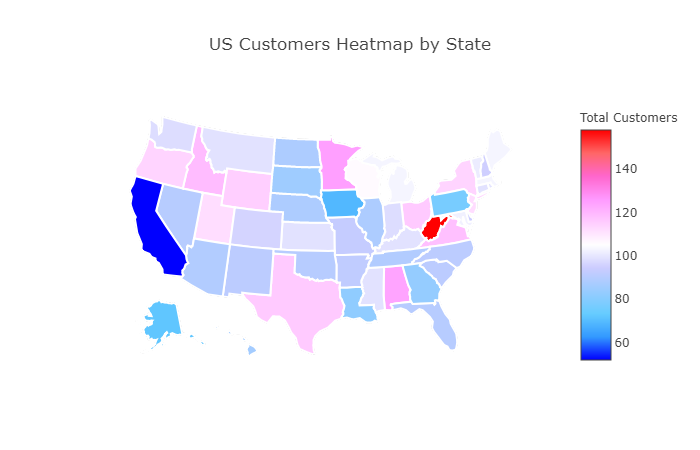
\includegraphics[scale = 0.5]{customers.png}
\caption{Customers Heatmap}
\label{fig:1.2}
\end{figure}
There are numerous customer in the North Eastern State of West Virgina and the least customers index being California.

\FloatBarrier
\subsection{Preprocessing}
All Machine Learning Algorithms take the data in a Guassian/Normal distribution for better prediction, accuracy and less variance among features. Eventhough, the most of the features are normally distributed we have scaled all the features for feeding data into model. The scaled data can be as shown 
\begin{figure}[h]
\vspace{-4pt}
\center
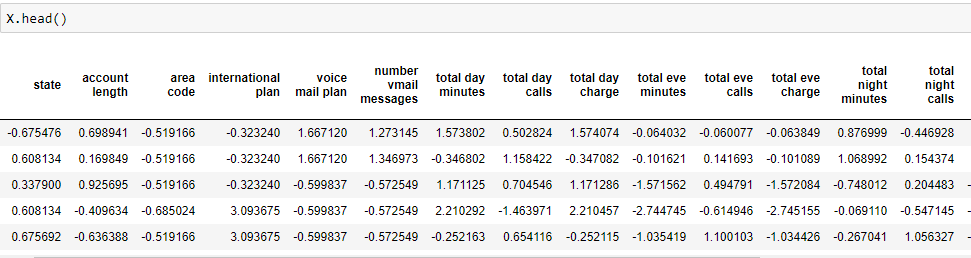
\includegraphics[scale = 0.5]{scaled_df.png}
\caption{Scaled data after preprocessing}
\label{fig:1.1}
\end{figure}
\FloatBarrier

\vspace{-05pt}
\chapter{Methodology}

\section{Preprocessing}
Data Exploration is an essential part of every Data Science project. The obtained data may not be always in the required form to perform any analysis or get insights. Most of the machine learining algorithms requires the data to be cleaned, processed or scaled to train a model on it. These techniques are easy to understand but every dataset is different and has a unique challenge in it.
\subsection{Outlier Analysis}

The shown boxplot Fig: \ref{fig:2.1} refers outliers on the predictors variables, we can see various outliers associated with the features. Eventhough, the data has considerale amount of outliers, the approach is to retain every outlier and grab respective behaviour of all customers. As shown there are significant amount of outliers present in the amount of night calls, which indicates a trend on customers' behaviour, there can be normal customers with an average usage appearing within the inter quartile, as well as customers who have business type accounts may have heavy usage and they appear above the quartile which seems important and can be concluded that Outliers here have information and retaining them would have advantage over the analysis.


\begin{figure}[htp]
\vspace{-70pt}
\center
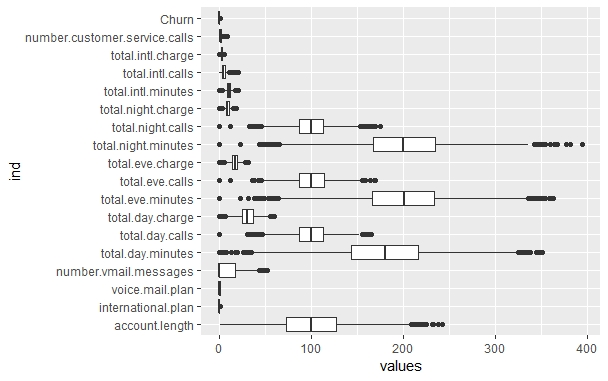
\includegraphics[width=\textwidth]{Boxplot.jpeg}
\caption{Boxplot on Predictors}
\label{fig:2.1}
\end{figure}
\FloatBarrier

\subsection{Feature Engineering}

Feature Engineering is described as the knowledge extraction process, where important features are selected using domain knowledge to make a machine learning algorithm work. There can be features that aren't relevant for the analysis, we can remove such variables using numerous ways. However, we considered taking correlation on the variables and make a heatmap Fig: \ref{fig:2.2} to check relationships among the features and then dropping redundant variables. 
\begin{figure}[h]
\vspace{-20pt}
\centering
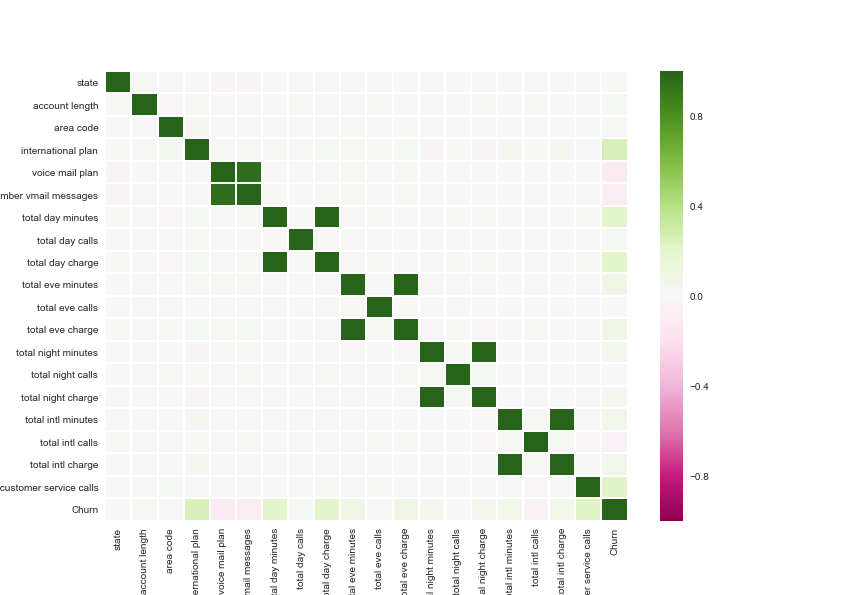
\includegraphics[scale = 0.4]{heatmap.png}
\caption{Heatmap on Predictors}
\label{fig:2.2}
\end{figure}
\FloatBarrier
\subsection{Feature Selection}
The Bi-Variate analysis in Fig: \ref{fig:2.3} shows International Plan, Total Day Minutes, Number of Customer Service Call are related with Churn which is shown in the Linear Plot  
\begin{figure}[h]
\vspace{-5pt}
\centering
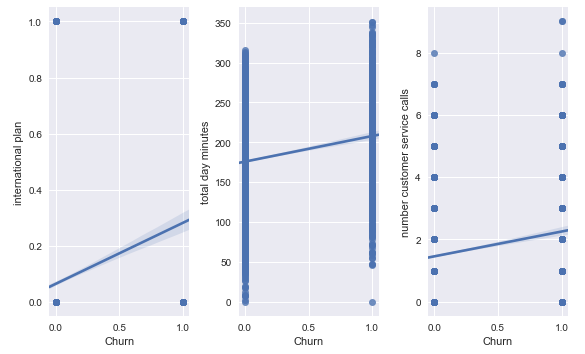
\includegraphics[scale = 0.7]{target_plot.PNG}
\caption{Univariate Analysis for Target Variables}
\label{fig:2.3}
\end{figure}
\FloatBarrier
The variables Number of Vmail Messages, Total Day Charge,Total Eve Charge,Total Night Charge,Total Intl Charge are dropped from the analysis as they are highly correlated with other variables.
The final variables selected for the analysis are Fig: \ref{fig:2.4}.
\begin{figure}[h]
\vspace{-5pt}
\centering
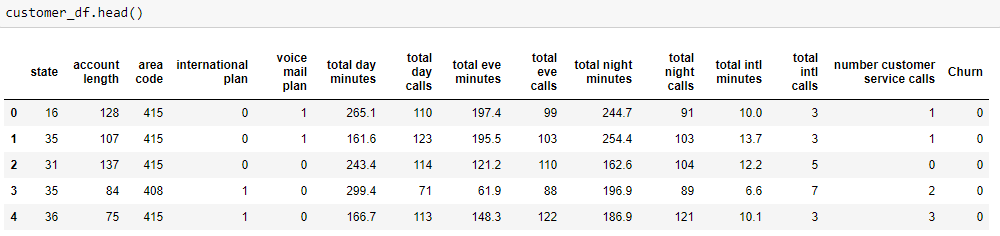
\includegraphics[scale = 0.5]{all_vars.PNG}
\caption{Selected Features for analysis}
\label{fig:2.4}
\end{figure}
\FloatBarrier
\chapter{Modeling}
\section{Ensemble Technique}
The goal of any machine learning problem is to find a single model that will best predict our wanted outcome. Rather than making one model and hoping this model is the best/most accurate predictor we can make, ensemble methods take a myriad of models into account, and average those models to select one final model. Our approach is to consider the classification models such as Logistic Regression, K-Nearest Neighbors, Decision Tree and The Random Forest model to obtain all the accuracies and then select a model that has a better Accuracy, Precision and Recall for a binomial prediction of whether or not a Customer will Churn. We used an iterative approach to test upon the above models and then plotted the results with accuracy,precision and recall respectively. The results from the model can be as shown,
\begin{figure}[h]
  \centering
  \begin{minipage}[b]{0.4\textwidth}
    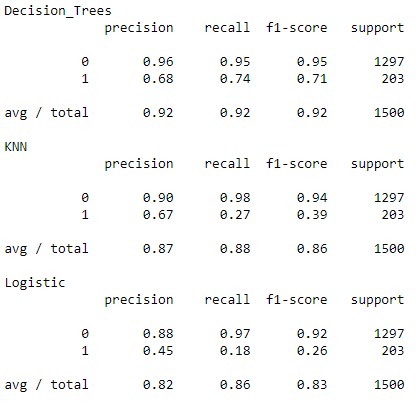
\includegraphics[width=\textwidth]{imb_model_results1.PNG}
     \caption{Model Results 3/4}
  \end{minipage}
  \hfill
  \begin{minipage}[b]{0.4\textwidth}
    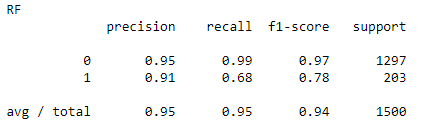
\includegraphics[width=\textwidth]{imb_results_2.PNG}
    \caption{Model Results 1/4}
  \end{minipage}
\end{figure}
Python code here: \\
\FloatBarrier


The results shows a good accuracy however the recall for these models are not acceptable as  we are more focused on the churning ratio and if the models predicts recall of 74\% for Decision Tree, 27\% for K-Nearest Neighbors, 18\% for Logistic Regression and 68\% for Random Forest Model. Which are relatively less and leads to the Type I Error which means the model gives irrelavant measure  in predicting that customers' churn however they don't  i.e; a minimum accuracy in predicting the False Positive Rate. The given ROC depicts the Area Under Curve for different models. All models didn't perform well and hence they fail to  give a better AUC.
\begin{figure}[h]
\vspace{-5pt}
\centering
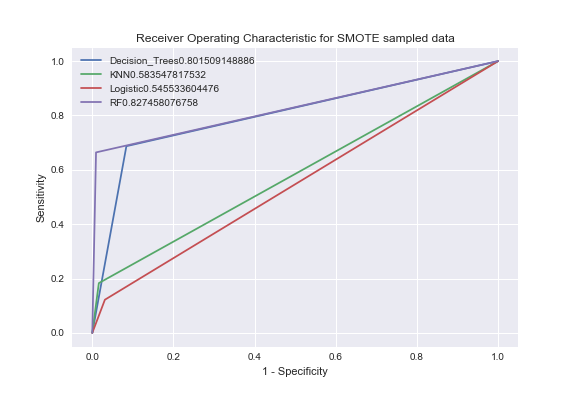
\includegraphics[scale = 0.7]{Imb_ROC.PNG}
\caption{Initial ROC plot(See Python Code Fig: \ref{lst:B.1})}
\label{fig:3.3}
\end{figure}
\FloatBarrier
Upon Re-Analysing we see that, the dataset is more biased towards the Customers who didn't Churned out then who did. Which leads to Target Class Imbalance in the dataset.
\section{Target Class Imbalance}
It is the problem in machine learning where the total number of a class of data (positive) is far less than the total number of another class of data (negative). This problem is extremely common in practice and can be observed in various disciplines.\\
Most machine learning algorithms and works best when the number of instances of each classes are roughly equal. When the number of instances of one class far exceeds the other, problems arise. This is best illustrated with our current situation.\\
In our dataset of Churn ratio, we would like to find out which are Customers that churned and who didn't. Now, it is highly cost effective for telecom company if a trusted customers churns, and costs a loss of a valuable customer. We want to catch as many cases of TRUE churning as possible and then optimize the parameters to reduce the TRUE churning ratio.\\
The imbalanced ratio as shown 
\begin{figure}[h]
\vspace{5pt}
\centering
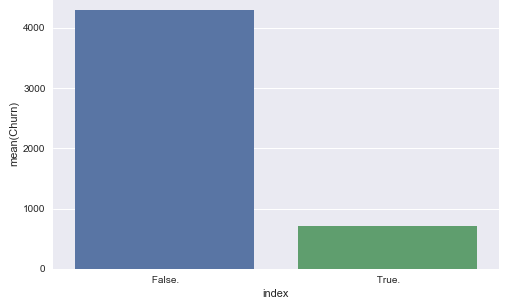
\includegraphics[scale = 0.7]{Target_imb.PNG}
\caption{Target Class Imbalance}
\label{fig:3.4}
\end{figure}
\FloatBarrier
\section{SMOTE for Reducing Imbalance}
Synthetic Minority Oversampling (SMOTE) is a technique which resamples the minority samples by selecting k nearest minority samples  and then creating a synthetic sample which equals to the average between two samples,  it's better option then replicating minority samples.\\
We will apply this sampling approach and check every models' performance. The R and Python implementations are as shown
\begin{lstlisting}[language=Python, caption=Python SMOTE Implementation]
from imblearn.over_sampling import SMOTE
sm = SMOTE(random_state = 101)
X_res, y_res = sm.fit_sample(X, y)
X_train, X_test, y_train, y_test = train_test_split(X_res, y_res, test_size=0.3, random_state=101) 
\end{lstlisting}
\FloatBarrier
\begin{lstlisting}[language=R, caption=R resampling]
#Creating over,under,both and synthetic samples to overcome target imbalance
cdf_over = ovun.sample(Churn ~., data = cdf_train, method = 'over',N = 5984)$data
cdf_under = ovun.sample(Churn ~., data = cdf_train, method = 'under',N = 1004)$data
cdf_both = ovun.sample(Churn ~., data = cdf_train, method = 'both',
                       p = 0.5,
                       seed = 221,
                       N = 3494)$data

cdf_ROSE = ROSE(Churn ~., data = cdf_train,
                N = 5000,
                seed = 221)$data
\end{lstlisting}
After Resampling the data we see that there is an equal distribution for both the categories in the response variable.
\begin{figure}[h]
\vspace{5pt}
\centering
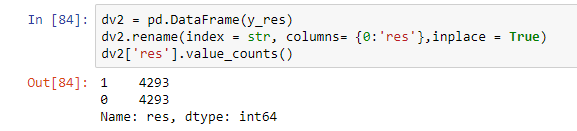
\includegraphics[scale = 0.7]{balanced.PNG}
\caption{Balanced resampled data}
\label{fig:3.5}
\end{figure}
\FloatBarrier
\section{Re-modeling with Balanced Set}
After resampling using the Synthetic Method the models are trained with the a balanced target class and hence the obatined ROC is as shown, which shows better AUC and the models perform well in determining the Recall and the Precision alongwith a better Accuracy. The RF model again shows  a better accuracy of 97\% while Logistic model with an acuuracy of 79\% being the least. The Receiver Operator Curve for these models is as shown \\
\begin{figure}[!htbp]
\vspace{-100pt}
\centering
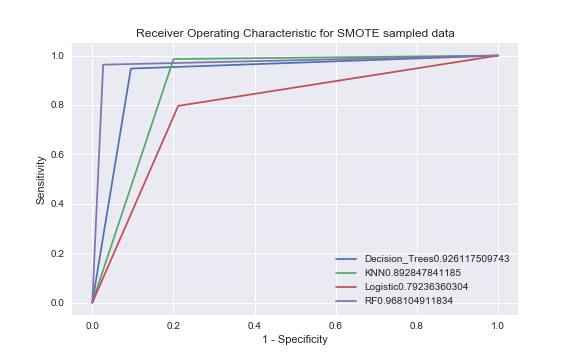
\includegraphics[width = \textwidth]{Balanced_ROC.PNG}
\caption{ROC on Balanced Data}
\label{fig:3.6}
\end{figure}
\FloatBarrier
The shown ROC curve depicts better performance with a balanced dataset. There is significant difference in both the ROC curve and we can conclude that Target Class Imbalance has made the model to perform with a better Recall and hence the aim of Reducing the Churn with a decent Recall solves the issue.


\chapter{Conclusion}
\section{Model Evaluation}
The metrics to evaluate a machine learning model is very important. Choice of metrics influences how the performance of machine learning algorithms is measured and compared. 
We can use classification performance metrics such as:\\
\textit{Log-Loss}\\
\textit{Accuracy}\\
\textit{AUC(Area under Curve)} etc\\
Another example of metric for evaluation of machine learning algorithms is precision, recall, which can be used for sorting algorithms primarily used by search engines.\\


\subsection{Precision}
With the evaluation on all the models we can conclude that our predictive performance parameter is the Precision Rate by which we can accurately predict the number of customers that will churn out.


\begin{lstlisting}[language=R, caption=RF performance]
> confusionMatrix(ConfMatrix_RF)
Confusion Matrix and Statistics

   RF_Predictions
       0    1
  0 1253    9
  1   40  173
                                          
               Accuracy : 0.9668          
                 95\% CI : (0.9563, 0.9753)
    No Information Rate : 0.8766          
    P-Value [Acc > NIR] : < 2.2e-16       
                                          
                  Kappa : 0.8569          
 Mcnemar's Test P-Value : 1.822e-05       
                                          
            Sensitivity : 0.9691          
            Specificity : 0.9505          
         Pos Pred Value : 0.9929          
         Neg Pred Value : 0.8122          
             Prevalence : 0.8766          
         Detection Rate : 0.8495          
   Detection Prevalence : 0.8556          
      Balanced Accuracy : 0.9598          
                                          
       'Positive' Class : 0           
\end{lstlisting}
Better predictions on the Churning ratio is obtained with the Random Forest Model and hence it can be selected as the final model to precisely predict upon the parameters to that can lead to the cancellation of service by a customer. 
\subsection{AUC/ROC}
The final model that can be perfectly classify among the two kinds of customer is the Random Forest Model.
\begin{figure}[!htbp]
\vspace{5pt}
\centering
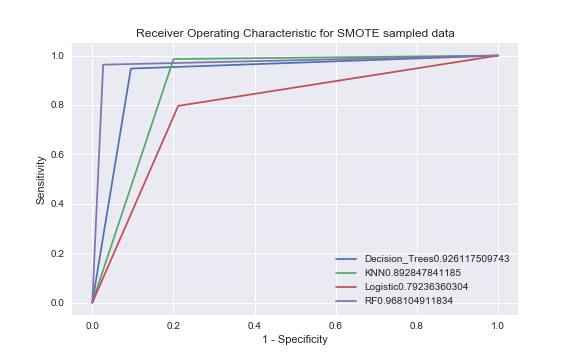
\includegraphics[scale = 0.5]{Balanced_ROC.PNG}
\caption{ROC on Balanced Data}
\label{fig:4.1}
\end{figure}
\FloatBarrier
\section{Model Selection}

With the obtained results we can say the model on Random FOrest is a decent predictor of the Churn Class and we can finalize  this model for the approach ROC Fig: \ref{fig:A.4} .
\subsection{Important Variables}
The important variables for the churn are:\\
1. Total day Minutes which relates to the day charges\\
2. International Plan\\
3. Number of Customer Service Calls\\
\begin{figure}[!htbp]
\vspace{5pt}
\centering
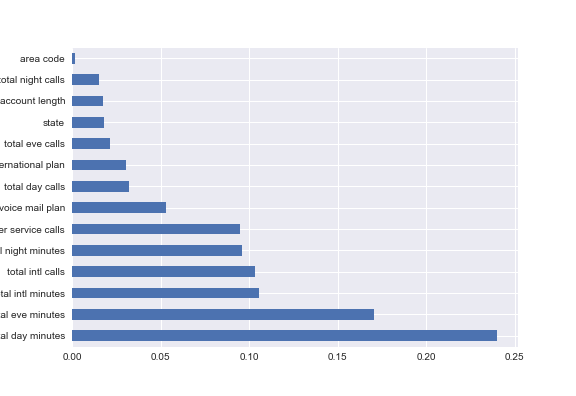
\includegraphics[scale = 0.5]{varz_imp.png}
\caption{Important Variables in Analysis}
\label{fig:4.2}
\end{figure}
\FloatBarrier
Python Code here: \ref{lst:B.7}

\appendix
\chapter{Extra Figures}
\begin{figure}[!htbp]
\vspace{-5pt}
\centering
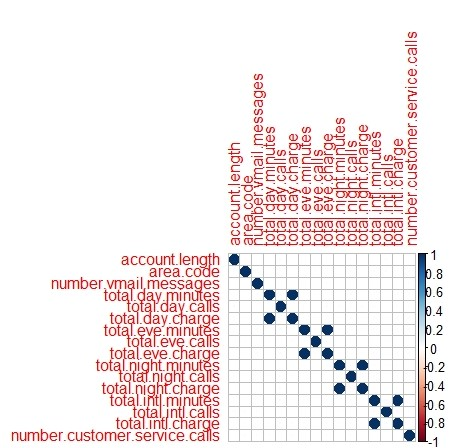
\includegraphics[scale = 1]{corrplot.jpeg}
\caption{R corrplot (See R code in appendix \ref{lst:B.5})}
\label{fig:A.1}
\end{figure}
\FloatBarrier

\begin{figure}[!htbp]
\vspace{-10pt}
\centering
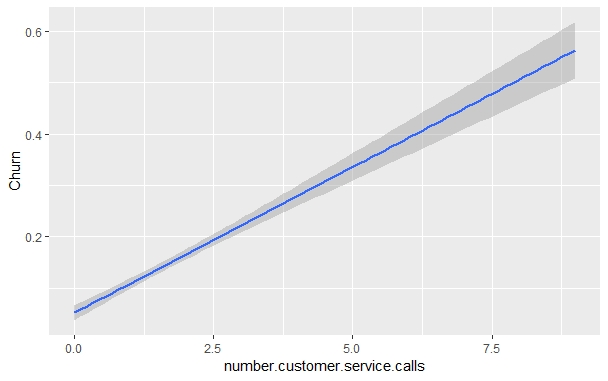
\includegraphics[scale = 0.6]{CustCallVsChurn.jpeg}
\caption{Linear Graph for relation with target variable (See R code in appendix \ref{lst:B.4})}
\label{fig:A.2}
\end{figure}
\FloatBarrier

\begin{figure}[!htbp]
\vspace{70pt}
\centering
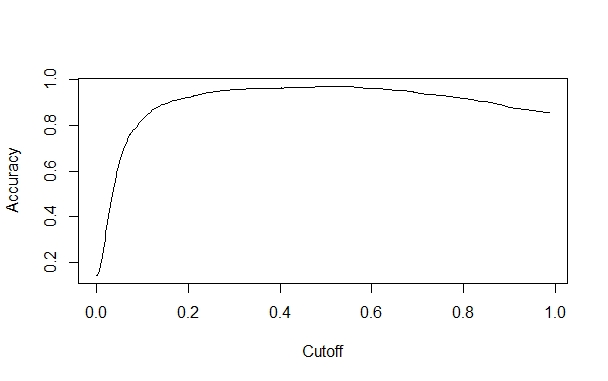
\includegraphics[scale = 0.6]{RoC_RandomForest.jpeg}
\caption{ROC for the Random Forest Model (See R code in appendix \ref{lst:B.2})}
\label{fig:A.3}
\end{figure}
\FloatBarrier

\begin{figure}[!htbp]
\vspace{-100pt}
\centering
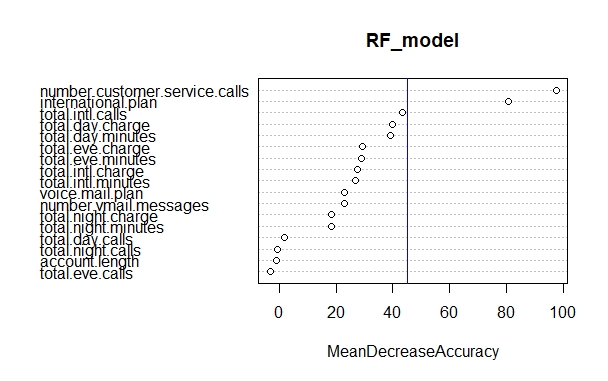
\includegraphics[width = \textwidth]{var_imp.jpeg}
\caption{Variable Importance for Random Forest(See R code in appendix \ref{lst:B.3})}
\label{fig:A.4}
\end{figure}
\FloatBarrier

\chapter{Code}

\begin{lstlisting}[language=Python, caption= Multiple ROC Model,label=lst:B.1]

model_predictions = [pred1,pred2,pred3,pred4] #list for every models predictions
models = ['Decision_Trees','KNN','Logistic','RF'] #list to specify the model names

#looping multiple models for plotting a single ROC Curve to evaluate models performance
for plots in range(0,4):
    fpr, tpr, thresh = metrics.roc_curve(y_test, model_predictions[plots])
    auc = metrics.roc_auc_score(y_test, model_predictions[plots])
    plt.plot(fpr,tpr,label=models[plots]+str(auc))
    plt.legend(loc=0)
    plt.xlabel('1 - Specificity')
    plt.ylabel('Sensitivity')
    plt.title('Receiver Operating Characteristic for SMOTE sampled data')
    print(models[plots])
    print(classification_report(y_test,model_predictions[plots]))
    plt.savefig('Balanced_ROC.png')
\end{lstlisting}
\FloatBarrier
\begin{lstlisting}[language=R, caption= RF ROC,label=lst:B.2]

#ROC Curve
RF_roc = predict(RF_model,cdf_test,type = 'prob')[,2]
RF_roc =  prediction(RF_roc,cdf_test$Churn)
eval_ = performance(RF_roc,'acc')
plot(eval_)

\end{lstlisting}
\FloatBarrier
\begin{lstlisting}[language=R, caption= RF ROC,label=lst:B.3]
#Variable Importance 
plot.new()
varImpPlot(RF_model,type = 1)
abline(v = 45, col= 'blue')
#This plot resembles the important parameters in RF prediction
\end{lstlisting}
\FloatBarrier
\begin{lstlisting}[language=R, caption= Relation Plot,label=lst:B.4]
# Correlation with the Target Variable
ggplot(customer_df, aes(x=international.plan, y=Churn)) +
  geom_point(shape=1) +    
  geom_smooth(method=lm)

ggplot(customer_df, aes(x=total.day.minutes, y=Churn)) +
  geom_smooth(method=lm)

ggplot(customer_df, aes(x=total.day.charge, y=Churn)) +
  geom_smooth(method=lm)

ggplot(customer_df, aes(x=number.customer.service.calls, y=Churn)) +
  geom_smooth(method=lm)
#All these plots shows a positive relation with the Target Variable 
\end{lstlisting}
\FloatBarrier
\begin{lstlisting}[language=R, caption=Correlation Plot,label=lst:B.5]
corrgram(customer_df, order = F, lower.panel = panel.shade,
         upper.panel=panel.pie, text.panel=panel.txt, main = "Correlation Plot")
\end{lstlisting} 
\begin{lstlisting}[language=Python, caption=US Heatmap,label=lst:B.6]
states = states_.value_counts()
state_ls = list(states.index)
state_vs = list(states.values)
import plotly.plotly as py
import plotly.graph_objs as go 
from plotly.offline import download_plotlyjs, init_notebook_mode, plot, iplot
init_notebook_mode(connected=True) 
data = dict(type='choropleth',
            colorscale = 'Picnic',
            locations = state_ls,
            z = state_vs,
            locationmode = 'USA-states',
            text = target,
            marker = dict(line = dict(color = 'rgb(255,255,255)',width = 2)),
            colorbar = {'title':"Total Customers"}
            )
layout = dict(title = 'US Customers Heatmap by State',
              geo = dict(scope='usa'))
choromap = go.Figure(data = [data],layout = layout)
iplot(choromap)
\end{lstlisting} 
\FloatBarrier
\begin{lstlisting}[language=Python, caption=Variable Importance,label=lst:B.7]
vars_ = (pd.Series(model_RF.feature_importances_, index=X.columns)
   .nlargest(14)
   .plot(kind='barh'))
plt.savefig('varz_imp.png')
\end{lstlisting} 
\end{document}



